\documentclass[12pt,english]{article}
\usepackage{geometry}
\usepackage{float}
\usepackage{caption}
\geometry{verbose,tmargin=3cm,bmargin=3cm,lmargin=3cm,rmargin=3cm}
\usepackage{amsmath}
\usepackage{amssymb}
\usepackage{amsthm}
\usepackage{verbatim}
\usepackage{adjustbox}
\usepackage{hyperref}
\usepackage{graphicx}
\usepackage{setspace}
\usepackage{changepage}
\onehalfspacing
\usepackage{babel}
\newcommand{\expec}{\ensuremath{\mathbb E}}
\begin{document}
\begin{center}
{\Large{}Section 10: Family size and education} \\
{\large{}Jayachandran and Pande (2015)}
\par\end{center}{\Large \par}

\begin{center}
EEP 152
\par\end{center}

\begin{center}
November 16, 2016
\par\end{center}

\begin{itemize}
	\setlength\itemsep{-0.5em}
	\item Economics of family size (10 min)
	\item Descriptive statistics on family size (30 min)
	\item JP (10 min)
\end{itemize}
A copy of a public version of the paper, along with the section notes, are available on the section Github at \href{github.com/johnloeser/eep152}{github.com/johnloeser/eep152} in the ``section10'' folder.

\section{Economics of family size}

Educational attainment and population dynamics are two important concepts in development economics. We've spend the past few weeks discussing the former, and the links between education and income. As to the latter, Malthus is famous for presenting the idea that people will have children until everyone is on the verge of starvation, which would be consistent with a model where children are costless and only benefit their parents. More recently, while modern agriculture has seemingly broken us free from the Malthusian trap, population growth still enters as an important parameter to the Solow growth model. In that framework, countries growing rapidly will have more difficultly accumulating capital while maintaining levels of consumption per capita. Finally, the two are linked, in that parents expend resources both to have children and to invest in the human capital of their children. In fact, this linkage can generate a poverty trap, where poor countries have fast population growth and invest little in human capital, while rich countries have slow population growth and invest intensively in human capital. Taken together, understanding the joint determination of human capital and population dynamics potentially provides a useful framework for understanding persistent gaps between poor and rich countries.

In class, we used a two period model, where parents trade off consumption in period 1 (while raising children) and period 2 (when they benefit from their children). Each child costs $\ell$ units of time and $c$ units of consumption in period 1. Additionally, each unit of the child's schooling $s$ costs 1 unit of consumption in period 1. Parents have an opportunity cost of time that's equivalent to $w_{1}$ units of consumption (which we can think of as their wage).

In period 2, children earn a wage $w_{2} (1 + rs)$. Additionally, each child supports their parent with probability $p$. This implies

$$ U(n, s) = \underbrace{u(w_{1}(1 - n \ell) - n(c + s))}_{\text{period 1 utility}} + \underbrace{\beta u(pnw_{2}(1 + rs))}_{\text{period 2 utility}} $$

How should parents trade off investments in number of children and schooling? In both cases, they receive a benefit in period 2, with a cost in period 1. In that sense, we can put this into a cost effectiveness framework, thinking about units of period 2 consumption gained per unit of period 1 consumption lost. Parents will make whichever investment has a higher cost effectiveness (or, will equate the marginal cost effectiveness of both investments). We can calculate the cost effectiveness of each using

$$ -\frac{\partial c_{2} / \partial n}{\partial c_{1} / \partial n} = \frac{pw_{2}(1 + rs)}{w_{1} \ell + c + s} $$
$$ -\frac{\partial c_{2} / \partial s}{\partial c_{1} / \partial s} = \frac{npw_{2}r}{n} = pw_{2}r $$

We can note a few implications. First, whether investments in education and having more children are complements or substitutes is ambiguous - higher optimal levels of schooling increases the cost of having children, but it also increases the benefits. As a result, the effects of increased $w_{2}$, which increases the cost effectiveness of schooling and having more children proportionally, but also increases period 2 income, is ambiguous. Second, increased $w_{1}$ reduces the cost effectiveness of having more children, but also increases income in period 1. Both of these effects will drive increased investment in education, but the effect on number of children is ambiguous. Third, increases in $r$ increase the relative cost effectiveness of schooling, but also increase period 2 income. This (likely) results in a decrease in number of children, and ambiguous effects on schooling.

What should we expect in practice? Vogl (2015) has a paper studying these patterns. He finds that historically, richer parents (high $w_{1}$) had more children, and their children got more education. This is consistent with high costs $c$ per child, which poor parents historically could not afford. More recently, the pattern has shifted, which richer parents (high $w_{1}$) having fewer children, but their children getting more education. This is consistent with a lower $c$ (or higher $p$ for poor families), as everyone's incomes generally rose (and children's probability of survival increased).

More recently, in some countries and demographic groups, we can now document another shift, where again richer parents have more children and their children get more education. This is potentially consistent with a rise in $r$, where poorer parents begin to invest more in their children's education, but this increases the costs of having a child, reducing the optimal number of children.

In sum, these patterns derive from decisions driven by many factors, and even this relatively complicated model is abstracting from a large number of factors. As a result, making predictions about correlations or effects of shocks is relatively hard. Additionally, some things outside the model we might also expect to have effects, such as the availability of contraception. However, the framework is a useful starting point for thinking about population dynamics and investment in education.

\section{Descriptive statistics on family size}

How can we test our model? Well, ideally we would find a natural experiment that generates variation in one of the determinants of family size. In a moment, we'll discuss a paper that makes use of the fact that Hindu parents generally live with their eldest son, and so compares differences in within family patterns of height-for-age and weight-for-age between India and sub-Saharan Africa, which potentially provides this sort of natural experiment (e.g. we can plausibly assume it's random whether your first two children are male-female or female-male if you have at least three children).

However, before trying to find a natural experiment, it is often useful to try to get a handle on basic correlations in order to understand the context. Although these are not causal, as we saw in the case of education, they often help us to understand what effects are potentially plausible and which aren't. Using ``familysize.R'' in the section GitHub, we'll look through World Bank WDI and a household survey dataset from Rwanda (EICV4) to explore these patterns.

\section{JP}

Jayachandran and Pande (2015) present a particularly interesting approach to studying the determination of investment in human capital by parents, allowing us to test the model. In particular, they present the puzzle that, relative to its income, the height of people in India is lower than in every sub-Saharan African country. Although one's initial instinct might be that this is driven by genetics, using household survey data, they show that this is driven by a steep gradient of height-for-age with respect to birth order: eldest children are taller in India than in sub-Saharan Africa, while second and third children in sub-Saharan Africa are taller than in India. This suggests differential investment in human capital (e.g. vaccinations, nutrition, investments in prenatal maternal health, \ldots) across the birth order in India relative to in sub-Saharan Africa.

\begin{figure}[H]
	\centering
	\begin{adjustbox}{width=\textwidth}
		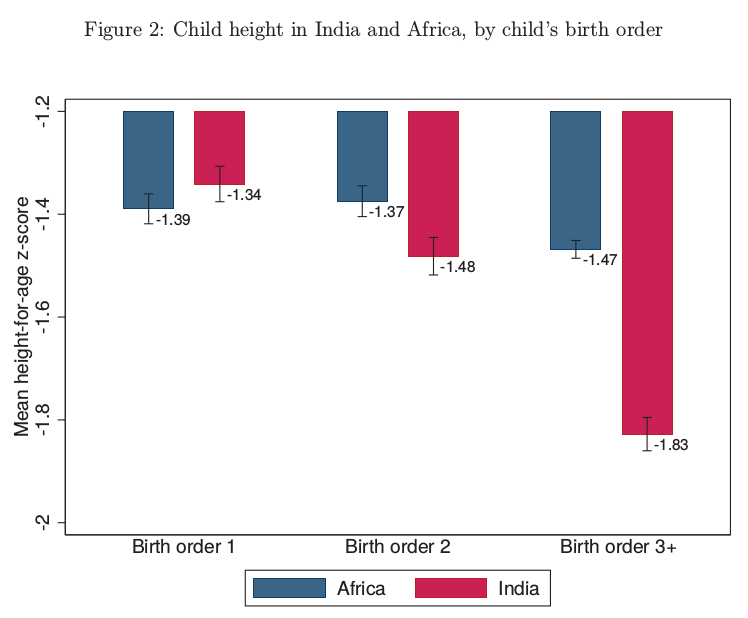
\includegraphics{fig1.png}
	\end{adjustbox}
\end{figure}

To explain this, they document that for many Hindus, the expectation is that the parents will live with their eldest son. As a result, the return (from the parents perspective) to investments in the human capital of their eldest son is much higher than for other children. In our model, this could be captures with $p$ being extremely high only for an eldest son, and much lower for other children. In that case, optimal investments in human capital for the eldest son would be higher than for other children.

To test this, they effectively run 2 DID specifications. In the first, they compare the height of eldest sons relative to eldest daughters, in India relative to in sub-Saharan Africa. In the second, they compare the height of eldest sons relative to second and third sons in India relative to in sub-Saharan Africa.

\begin{figure}[H]
	\centering
	\begin{adjustbox}{width=\textwidth}
		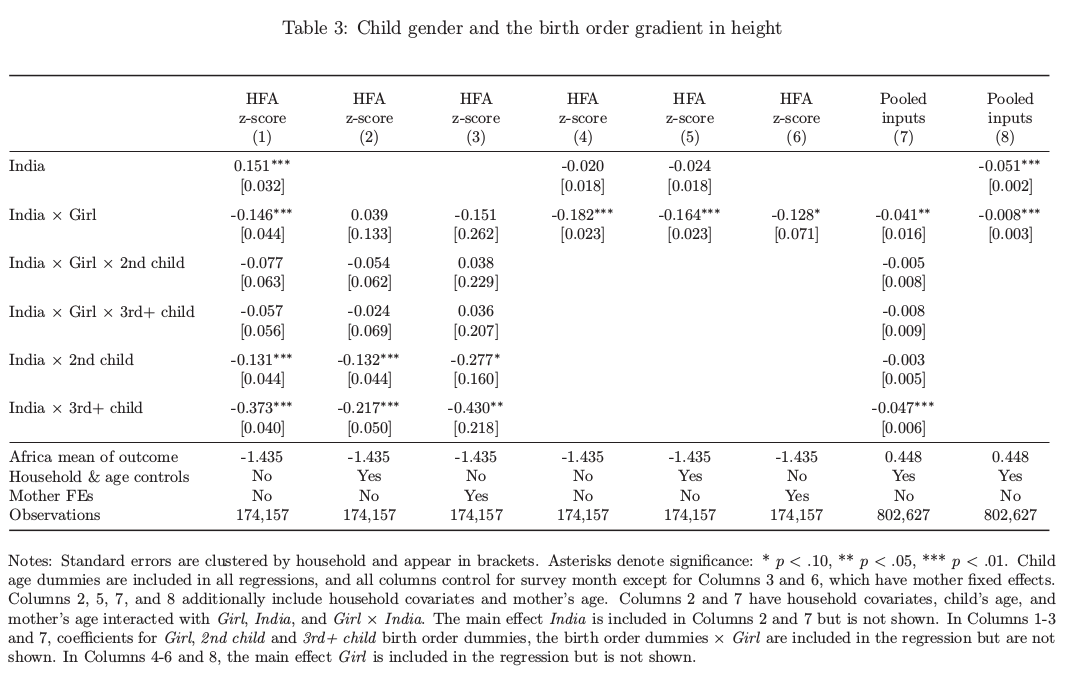
\includegraphics{fig2.png}
	\end{adjustbox}
\end{figure}

\newpage
How do we interpret these regression coefficients? It's useful to think about this as six sets of comparisons -- eldest, second, and third+ sons and daughters in India relative to the eldest, second, and third+ sons and daughters in sub-Saharan Africa. We can add the appropriate coefficients up to plot each of these differences separately.

\begin{figure}[H]
	\centering
	\begin{adjustbox}{width=\textwidth}
		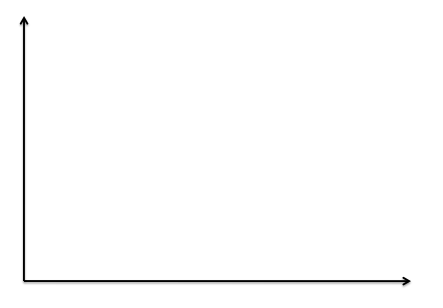
\includegraphics{axes.png}
	\end{adjustbox}
\end{figure}

\end{document}